\documentclass[aspectratio=169]{beamer}

% Professional Academic Theme
\usetheme{Madrid}
\usecolortheme{default}

% Packages
\usepackage{amsmath,amsfonts}
\usepackage[english]{babel}
\usepackage{tikz}
\usepackage{pgfplots}
\pgfplotsset{compat=1.18}

% Information
\title{Time Series}
\subtitle{Non-Stationary Time Series \& Volatility Models}
\author{Mr. Aymen Ben Brik}

\institute{
Time Series Course 1GAMMA
}

\date{\today}

\usepackage{listings}
\usepackage{xcolor}

\lstset{
language=Python,
basicstyle=\ttfamily\small,
keywordstyle=\color{blue},
commentstyle=\color{gray},
stringstyle=\color{red},
showstringspaces=false,
frame=single,
breaklines=true
}

\begin{document}

% Title Slide
\begin{frame}
\titlepage
\end{frame}

% Title Slide
\begin{frame}
\tableofcontents
\end{frame}

% Objectives
\begin{frame}{Session Objectives}
\begin{itemize}
    \item Understand the limitations of the stationarity assumption in real-world data
    \item Master the fundamental mathematical operators: Backshift ($B$) and Differencing ($\Delta$)
    \item Model non-stationary and seasonal time series using ARIMA and SARIMA processes
    \item Understand the concept of volatility clustering in financial time series
    \item Apply ARCH and GARCH models to capture conditional heteroscedasticity
\end{itemize}
\end{frame}

\section{Introduction to Non-Stationarity}

\begin{frame}{Limits of the Stationarity Assumption}
\begin{itemize}
    \item \textbf{Recall - Weak Stationarity:} Assumes the statistical properties of the series (mean $\mu$, variance $\sigma^2$, and autocovariance) remain constant over time.
    \vspace{0.2cm}
    \item \textbf{The Reality of Real-World Data:} Most macroeconomic and financial series (e.g., GDP, stock prices, exchange rates) violate these assumptions.
    \vspace{0.2cm}
    \item They frequently exhibit:
    \begin{itemize}
        \item Changing levels or trends (non-constant mean).
        \item Structural breaks or seasonality.
        \item Periods of high and low volatility (non-constant variance).
    \end{itemize}
    \vspace{0.2cm}
    \item \textbf{Implication:} Applying standard ARMA models directly to such data yields invalid inferences and poor forecasts; transformations are strictly necessary.
\end{itemize}
\end{frame}

\begin{frame}{Types of Non-Stationarity}
\begin{itemize}
    \item \textbf{Deterministic Trend:}
    \begin{itemize}
        \item The series evolves around a predictable, fixed function of time.
        \item Example (Linear): $X_t = \alpha + \beta t + \varepsilon_t$
        \item Shocks ($\varepsilon_t$) are temporary; the series always reverts to its underlying trend.
        \item \textbf{Solution:} Detrending (e.g., subtracting an estimated OLS regression line).
    \end{itemize}
    
    \vspace{0.4cm}
    
    \item \textbf{Stochastic Trend (Unit Root):}
    \begin{itemize}
        \item The series does not fluctuate around a fixed level; its variance grows indefinitely over time.
        \item Example (Random Walk): $X_t = X_{t-1} + \varepsilon_t$
        \item Shocks ($\varepsilon_t$) have a \textbf{permanent} effect; the series has no memory of a "mean" to revert to.
        \item \textbf{Solution:} Differencing (applying the $\Delta$ operator to achieve stationarity).
    \end{itemize}
\end{itemize}
\end{frame}

\begin{frame}{Consequences of Non-Stationarity}
\begin{itemize}
    \item \textbf{Spurious Regressions:} 
    \begin{itemize}
        \item Regressing two completely independent non-stationary series (e.g., two unrelated random walks) often yields a high $R^2$ and highly significant t-statistics.
        \item This falsely suggests a strong economic relationship where none actually exists.
    \end{itemize}
    
    \vspace{0.4cm}
    
    \item \textbf{Invalid Statistical Inference:}
    \begin{itemize}
        \item Standard Ordinary Least Squares (OLS) assumptions are violated.
        \item Test statistics (t-tests, F-tests) do not follow their standard distributions, making p-values misleading and hypothesis testing unreliable.
    \end{itemize}
    
    \vspace{0.4cm}
    
    \item \textbf{Unreliable Forecasting:}
    \begin{itemize}
        \item For processes with a stochastic trend (unit root), the effect of past shocks does not decay over time.
        \item The variance of the forecast error grows indefinitely, making long-term predictions virtually meaningless.
    \end{itemize}
\end{itemize}
\end{frame}

\section{Fundamental Mathematical Operators}

\begin{frame}{The Backshift Operator ($B$)}
\textbf{Definition:}
\[
B X_t = X_{t-1}
\]

\textbf{Properties:}
\begin{itemize}
    \item \textbf{Recursive Application:} Applying the operator $k$ times shifts the time index back by $k$ periods.
    \[ B^k X_t = X_{t-k} \]
    
    \vspace{0.2cm}
    
    \item \textbf{Algebraic Manipulation:} The operator $B$ behaves like a standard mathematical variable. We can add, multiply, and factor polynomials in $B$ to simplify complex equations.
    \begin{itemize}
        \item \textit{Example for an AR(1) process:} $X_t = \phi X_{t-1} + \varepsilon_t$
        \item Rewrite using $B$: $X_t = \phi B X_t + \varepsilon_t$
        \item Rearrange and factor: $(1 - \phi B)X_t = \varepsilon_t$
    \end{itemize}
\end{itemize}
\end{frame}

\begin{frame}{The Difference Operator ($\Delta$)}
\textbf{Definition of First Difference:}
\[
\Delta X_t = X_t - X_{t-1} = (1 - B)X_t
\]

\textbf{Connection to Trend Elimination:}
\begin{itemize}
    \item \textbf{Purpose:} The first difference is primarily used to eliminate a \textbf{linear trend} or a \textbf{stochastic trend} (random walk), stabilizing the mean of the series.
    \vspace{0.2cm}
    \item \textbf{Mathematical Intuition (Linear Trend):}
    \begin{itemize}
        \item Suppose a series has a linear trend: $X_t = \alpha + \beta t + \varepsilon_t$
        \item Applying the first difference:
        \[ \Delta X_t = (\alpha + \beta t + \varepsilon_t) - (\alpha + \beta(t-1) + \varepsilon_{t-1}) \]
        \[ \Delta X_t = \beta + \Delta \varepsilon_t \]
        \item \textbf{Result:} The time-dependent variable $t$ is completely eliminated, leaving a stationary process with a constant mean ($\beta$).
    \end{itemize}
\end{itemize}
\end{frame}


\begin{frame}{Higher-Order Differencing ($d$)}
\textbf{Formulation:}
\[
\Delta^d X_t = (1 - B)^d X_t
\]

\textbf{Geometric Intuition \& Application:}
\begin{itemize}
    \item The order of differencing ($d$) corresponds to the polynomial degree of the trend being eliminated.
    \vspace{0.2cm}
    \item \textbf{$d=1$ (First Difference):} Eliminates a \textbf{linear trend} (analogous to velocity or constant rate of change).
    \item \textbf{$d=2$ (Second Difference):} Eliminates a \textbf{quadratic trend} (analogous to acceleration).
    \begin{itemize}
        \item Algebraic expansion: 
        \[ \Delta^2 X_t = (1 - B)^2 X_t = (1 - 2B + B^2) X_t = X_t - 2X_{t-1} + X_{t-2} \]
    \end{itemize}
    \vspace{0.3cm}
    \item \textbf{Practical Rule of Thumb:}
    \begin{itemize}
        \item In practice, it is extremely rare to use $d > 2$.
        \item \textbf{Warning:} \textit{Over-differencing} a series introduces artificial serial correlation (moving average noise) and makes model estimation much harder. Always stop differencing as soon as stationarity is reached.
    \end{itemize}
\end{itemize}
\end{frame}
\begin{frame}[fragile]{Implementation in R: Backshift and Differencing}
\small
\textbf{Goal:} Apply the $B$ and $\Delta$ operators using R.

\vspace{0.2cm}

\begin{columns}[T]
\begin{column}{0.48\textwidth}
\begin{block}{Backshift Operator ($B$)}
\begin{verbatim}
# Using the dplyr package for lag
library(dplyr)

# Original series
x <- c(10, 15, 12, 18)

# Apply Backshift B(X_t) = X_{t-1}
B_x <- lag(x, n = 1)

print(B_x)
# Output: NA 10 15 12
\end{verbatim}
\end{block}
\end{column}

\begin{column}{0.48\textwidth}
\begin{block}{Difference Operator ($\Delta$)}
\begin{verbatim}
# Using base R

# Original series
x <- c(10, 15, 12, 18)

# Apply Difference \Delta(X_t)
delta_x <- diff(x, differences = 1)

print(delta_x)
# Output: 5 -3 6
\end{verbatim}
\end{block}
\end{column}
\end{columns}

\vspace{0.3cm}
\textbf{Note:} \texttt{diff()} reduces the length of the vector by 1, whereas \texttt{lag()} keeps the same length but introduces an \texttt{NA} at the beginning.
\end{frame}

\begin{frame}[fragile]{Implementation in Python: Backshift and Differencing}
\small
\textbf{Goal:} Apply the $B$ and $\Delta$ operators using Python (Pandas).
\begin{columns}[T]
\begin{column}{0.48\textwidth}
\begin{block}{Backshift Operator ($B$)}
\begin{verbatim}
import pandas as pd

# Original series
x = pd.Series([10, 15, 12, 18])
# Apply Backshift B(X_t) = X_{t-1}
B_x = x.shift(1)
print(B_x.tolist())
# Output: [nan, 10.0, 15.0, 12.0]
\end{verbatim}
\end{block}
\end{column}

\begin{column}{0.48\textwidth}
\begin{block}{Difference Operator ($\Delta$)}
\begin{verbatim}
import pandas as pd

# Original series
x = pd.Series([10, 15, 12, 18])

# Apply Difference \Delta(X_t)
delta_x = x.diff(periods=1)

print(delta_x.tolist())
# Output: [nan, 5.0, -3.0, 6.0]
\end{verbatim}
\end{block}
\end{column}
\end{columns}

\vspace{0.3cm}
\textbf{Note:} Pandas naturally handles the alignment and retains the original length of the Series by inserting a \texttt{NaN} (Not a Number) for the first observation in both operations.
\end{frame}

\section{ARIMA Processes}

\begin{frame}{Intuition behind ARIMA(p,d,q)}
\begin{itemize}
    \item \textbf{The 'I' for Integrated:} Unlike standard ARMA models that require the data to be stationary from the start, ARIMA is designed for non-stationary data by \textit{integrating} the differencing step directly into the model.
    
    \vspace{0.2cm}
    
    \item \textbf{The Principle of Differencing ($d$):} If the original series $X_t$ exhibits a stochastic trend, we apply the difference operator $d$ times ($\Delta^d$) until it becomes a weakly stationary series.
    
    \vspace{0.2cm}
    
    \item \textbf{The ARMA Phase ($p, q$):} Once we obtain a stationary series $Y_t = \Delta^d X_t$, we capture its remaining short-term dynamics using Autoregressive (AR of order $p$) and Moving Average (MA of order $q$) components.
    
    \vspace{0.2cm}
    
    \item \textbf{Synthesis:} Simply put, an ARIMA($p, d, q$) model on the original series $X_t$ is just an ARMA($p, q$) model applied to the differenced series $\Delta^d X_t$.
\end{itemize}
\end{frame}

\begin{frame}{Mathematical Formulation}
\textbf{General Equation:}
\[
\Phi(B)\Delta^d X_t = \Theta(B)\varepsilon_t
\]

\textbf{Components of the Equation:}
\begin{itemize}
    \item \textbf{The AR Polynomial $\Phi(B)$:}
    \[ \Phi(B) = 1 - \phi_1 B - \phi_2 B^2 - \dots - \phi_p B^p \]
    \begin{itemize}
        \item Captures the \textbf{Autoregressive} component of order $p$.
        \item It models how the current differenced value depends linearly on its own $p$ past values.
    \end{itemize}
    
    \vspace{0.2cm}
    
    \item \textbf{The MA Polynomial $\Theta(B)$:}
    \[ \Theta(B) = 1 + \theta_1 B + \theta_2 B^2 + \dots + \theta_q B^q \]
    \begin{itemize}
        \item Captures the \textbf{Moving Average} component of order $q$.
        \item It models how the current value is impacted by $q$ past white noise shocks ($\varepsilon_{t-k}$).
    \end{itemize}
\end{itemize}
\end{frame}

\begin{frame}{Mathematical Example: Deriving an ARIMA(1,1,1)}
\textbf{Goal:} Expand the general equation for $p=1, d=1, q=1$.

\vspace{0.2cm}

\textbf{1. Define the specific components:}
\begin{itemize}
    \item AR(1) polynomial: $\Phi(B) = 1 - \phi_1 B$
    \item Integration ($d=1$): $\Delta = 1 - B$
    \item MA(1) polynomial: $\Theta(B) = 1 + \theta_1 B$
\end{itemize}

\vspace{0.2cm}

\textbf{2. Substitute into the general equation:}
\[
(1 - \phi_1 B)(1 - B)X_t = (1 + \theta_1 B)\varepsilon_t
\]

\vspace{0.2cm}

\textbf{3. Expand the left-hand side (LHS):}
\[
(1 - B - \phi_1 B + \phi_1 B^2)X_t = X_t - X_{t-1} - \phi_1 X_{t-1} + \phi_1 X_{t-2}
\]

\vspace{0.2cm}

\textbf{4. Final equation (isolating $X_t$):}
\[
X_t = (1 + \phi_1)X_{t-1} - \phi_1 X_{t-2} + \varepsilon_t + \theta_1 \varepsilon_{t-1}
\]

\end{frame}

\begin{frame}{Box-Jenkins Methodology Revisited}
\begin{enumerate}
    \item \textbf{Identification:} 
    \begin{itemize}
        \item \textbf{Determine $d$:} Use unit root tests (ADF, KPSS) to check for stationarity. Apply differencing ($\Delta$) until the series is weakly stationary.
        \item \textbf{Determine $p$ and $q$:} Analyze the Autocorrelation Function (ACF) and Partial Autocorrelation Function (PACF) of the \textit{differenced} series ($\Delta^d X_t$) to identify the AR and MA orders.
    \end{itemize}
    
    \vspace{0.3cm}
    
    \item \textbf{Estimation:} 
    \begin{itemize}
        \item Estimate the parameters ($\phi_1 \dots \phi_p, \theta_1 \dots \theta_q$) usually via Maximum Likelihood Estimation (MLE).
        \item Compare candidate models using Information Criteria (AIC, BIC) to balance goodness-of-fit with parsimony.
    \end{itemize}
    
    \vspace{0.3cm}
    
    \item \textbf{Diagnostic Checking:} 
    \begin{itemize}
        \item Analyze the residuals: they must behave like White Noise.
        \item Verify that the ACF of the residuals is flat and use the \textbf{Ljung-Box test} to ensure no significant serial correlation remains. If it fails, go back to Step 1.
    \end{itemize}
\end{enumerate}
\end{frame}

\begin{frame}[fragile]{Automated Model Selection: auto.arima in R}
\small
\textbf{Goal:} Automatically find the optimal ARIMA orders $(p,d,q)$ by minimizing Information Criteria (like AIC or BIC).

\vspace{0.2cm}

\begin{block}{R Implementation (\texttt{forecast} package)}
\begin{verbatim}
# Load the required package
library(forecast)

# Assuming 'ts_data' is a time series object
# Fit the best ARIMA model automatically (strictly non-seasonal)
best_model <- auto.arima(ts_data, 
                         seasonal = FALSE, 
                         stepwise = TRUE, 
                         trace = TRUE) # Shows the search process

# Display the selected model and its parameters
summary(best_model)
\end{verbatim}
\end{block}
\end{frame}

\begin{frame}[fragile]{Automated Model Selection: auto.arima in R}
\vspace{0.2cm}
\textbf{Key Warning:} \texttt{auto.arima} is a powerful shortcut, but it is not magic! You must still manually perform diagnostic checking on the residuals (e.g., Ljung-Box test) to ensure the selected model is valid.
\end{frame}

\begin{frame}[fragile]{Automated Model Selection: auto\_arima in Python}
\small
\textbf{Goal:} The Python equivalent of R's automated selection, utilizing the \texttt{pmdarima} library.

\vspace{0.2cm}

\begin{block}{Python Implementation (\texttt{pmdarima} package)}
\begin{verbatim}
# Install via terminal: pip install pmdarima
import pmdarima as pm

# Assuming 'data' is a pandas Series
# Fit the best ARIMA model automatically (strictly non-seasonal)
best_model = pm.auto_arima(data, 
                           seasonal=False, 
                           stepwise=True, 
                           trace=True,
                           error_action='ignore', 
                           suppress_warnings=True)

# Display the detailed model summary
print(best_model.summary())
\end{verbatim}
\end{block}
\end{frame}

\begin{frame}[fragile]{Automated Model Selection: auto\_arima in Python}

\vspace{0.2cm}
\textbf{Note:} By setting \texttt{seasonal=False}, the algorithm skips the search for $P, D, Q$ parameters and restricts its optimization strictly to the standard ARIMA$(p,d,q)$ framework.
\end{frame}
\section{SARIMA Processes}

\begin{frame}{The Problem of Seasonality}
\textbf{The Seasonal Difference Operator:}
\[
\Delta_s X_t = X_t - X_{t-s} = (1 - B^s)X_t
\]

\textbf{Why standard differencing ($\Delta$) is not enough:}
\begin{itemize}
    \item \textbf{Local vs. Periodic Focus:} Standard differencing ($\Delta = 1 - B$) only removes local, short-term trends by comparing adjacent periods (e.g., $t$ vs. $t-1$).
    
    \vspace{0.2cm}
    
    \item \textbf{Residual Seasonality:} If data has a strong periodic pattern (e.g., retail sales consistently spiking every December), comparing December to November ($\Delta X_t$) will yield a massive, repeating spike. The seasonal structure remains entirely intact.
    
    \vspace{0.2cm}
    
    \item \textbf{The Solution ($\Delta_s$):} To achieve true stationarity, we must compare "apples to apples". The seasonal operator $\Delta_s$ neutralizes the periodic effect by comparing the current observation strictly to its exact counterpart from the previous cycle (e.g., this December vs. last December).
\end{itemize}
\end{frame}

\begin{frame}{The SARIMA Model}
\textbf{Notation:} SARIMA$(p,d,q) \times (P,D,Q)_s$

\textbf{Understanding the Parameters:}
\begin{itemize}
    \item \textbf{Non-Seasonal Part $(p,d,q)$:} Models the standard, short-term dependencies (e.g., how yesterday affects today).
    
    \vspace{0.2cm}
    
    \item \textbf{Seasonal Part $(P,D,Q)$:} Models the periodic, long-term dependencies (e.g., how last December affects this December).
    \begin{itemize}
        \item $P$: Order of the Seasonal Autoregressive component.
        \item $D$: Number of Seasonal Differences applied.
        \item $Q$: Order of the Seasonal Moving Average component.
    \end{itemize}
    
    \vspace{0.2cm}
    
    \item \textbf{Seasonal Frequency ($s$):} Defines the length of the cycle.
    \begin{itemize}
        \item $s = 12$ for monthly data (yearly cycle).
        \item $s = 4$ for quarterly data.
        \item $s = 52$ for weekly data.
    \end{itemize}
\end{itemize}
\end{frame}

\begin{frame}{Intuition: Seasonal Orders $P=2$ and $Q=2$}
\textbf{Context:} What does it physically mean to have $P=2$ and $Q=2$ in a SARIMA model?

\vspace{0.2cm}
\begin{itemize}
    \item \textbf{Seasonal AR Order ($P=2$):}
    \begin{itemize}
        \item The current value depends directly on the actual observations from exactly \textbf{one and two full seasons ago}.
        \item \textit{Math:} $X_t$ is linearly dependent on $X_{t-s}$ and $X_{t-2s}$.
        \item \textit{Example ($s=12$):} This December's sales are predicted based on the sales from \textit{last} December and the December \textit{before that}.
    \end{itemize}
    
    \vspace{0.3cm}
    
    \item \textbf{Seasonal MA Order ($Q=2$):}
    \begin{itemize}
        \item The current value is impacted by the \textbf{unpredictable shocks (errors)} that occurred exactly one and two seasons ago.
        \item \textit{Math:} $X_t$ is influenced by $\varepsilon_{t-s}$ and $\varepsilon_{t-2s}$.
        \item \textit{Example ($s=12$):} An unexpected supply shortage last December ($\varepsilon_{t-12}$) and a massive snowstorm the December prior ($\varepsilon_{t-24}$) left residual impacts that still affect this December's forecast.
    \end{itemize}
\end{itemize}
\end{frame}

\begin{frame}{General SARIMA Equation}
\[
\Phi_P(B^s) \phi_p(B) \Delta_s^D \Delta^d X_t = \Theta_Q(B^s) \theta_q(B) \varepsilon_t
\]

\textbf{Combining Regular and Seasonal Components:}
\begin{itemize}
    \item \textbf{Multiplicative Structure:} SARIMA is a multiplicative model. The seasonal polynomials (uppercase) and non-seasonal polynomials (lowercase) are multiplied together to capture complex dynamics.
    
    \vspace{0.3cm}
    
    \item \textbf{Left-Hand Side (LHS) - The Series ($X_t$):}
    \begin{itemize}
        \item We apply standard differencing ($\Delta^d$) and seasonal differencing ($\Delta_s^D$) to make the series stationary.
        \item The resulting series is modeled by combining the short-term AR memory ($\phi_p$) and the long-term seasonal AR memory ($\Phi_P$).
    \end{itemize}
    
    \vspace{0.3cm}
    
    \item \textbf{Right-Hand Side (RHS) - The Shocks ($\varepsilon_t$):}
    \begin{itemize}
        \item The current value is impacted by a combination of recent white noise shocks (via $\theta_q$) and shocks that occurred exactly in previous seasons (via $\Theta_Q$).
    \end{itemize}
\end{itemize}
\end{frame}

\begin{frame}{Mathematical Example: SARIMA(1,1,1)$\times$(1,1,1)$_{12}$}
\textbf{Goal:} Write the equation for a monthly SARIMA model ($s=12$).

\vspace{0.2cm}

\textbf{1. Define the specific components:}
\begin{itemize}
    \item Non-seasonal AR/MA: $(1 - \phi_1 B)$ and $(1 + \theta_1 B)$
    \item Seasonal AR/MA: $(1 - \Phi_1 B^{12})$ and $(1 + \Theta_1 B^{12})$
    \item Differencing ($d=1, D=1$): $(1 - B)$ and $(1 - B^{12})$
\end{itemize}

\vspace{0.2cm}

\textbf{2. The Multiplicative Equation:}
\[
(1 - \Phi_1 B^{12})(1 - \phi_1 B)(1 - B^{12})(1 - B) X_t = (1 + \Theta_1 B^{12})(1 + \theta_1 B) \varepsilon_t
\]

\vspace{0.2cm}

\textbf{3. Key Insight: The Cross-Terms ($B^{13}$)}
\begin{itemize}
    \item Let's expand just the right-hand side (MA components):
    \[ RHS = (1 + \theta_1 B + \Theta_1 B^{12} + \theta_1 \Theta_1 B^{13}) \varepsilon_t \]
    \[ RHS = \varepsilon_t + \theta_1 \varepsilon_{t-1} + \Theta_1 \varepsilon_{t-12} + \theta_1 \Theta_1 \varepsilon_{t-13} \]
    \item \textbf{Interpretation:} The multiplicative structure automatically creates an interaction effect. The series is impacted by yesterday's shock, last year's shock, \textbf{and} a combined cross-shock from exactly 13 months ago.
\end{itemize}
\end{frame}

\begin{frame}{Practical Identification}
\textbf{Identifying Seasonal Orders ($P$ and $Q$):}
\begin{itemize}
    \item \textbf{Focus on Seasonal Lags:} To identify the seasonal components, we ignore the early lags (1, 2, 3...) and examine the behavior of the ACF and PACF strictly at multiples of the seasonal period ($s, 2s, 3s, \dots$).
    
    \vspace{0.3cm}
    
    \item \textbf{Identifying Seasonal MA ($Q$):}
    \begin{itemize}
        \item Look at the \textbf{ACF}. If there is a significant spike at lag $s$ (and perhaps $2s$), but it cuts off sharply to zero at subsequent seasonal lags, this indicates a Seasonal MA component.
        \item \textit{Example ($s=12$):} Significant ACF spike at lag 12, but nothing at lag 24 $\implies Q=1$.
    \end{itemize}
    
    \vspace{0.3cm}
    
    \item \textbf{Identifying Seasonal AR ($P$):}
    \begin{itemize}
        \item Look at the \textbf{PACF}. If there is a significant spike at lag $s$ and it cuts off sharply afterwards, while the ACF decays gradually across the seasonal lags, this indicates a Seasonal AR component.
        \item \textit{Example ($s=12$):} Significant PACF spike at lag 12, but nothing at lag 24 $\implies P=1$.
    \end{itemize}
\end{itemize}
\end{frame}

\begin{frame}{Visualizing Seasonal Signatures: SAR(1) with $s=12$}
\textbf{Case 1: Pure Seasonal Autoregressive Model ($P=1$)}

\vspace{0.2cm}
\begin{columns}[T]
\begin{column}{0.5\textwidth}
\begin{center}
\textbf{Theoretical ACF} \\
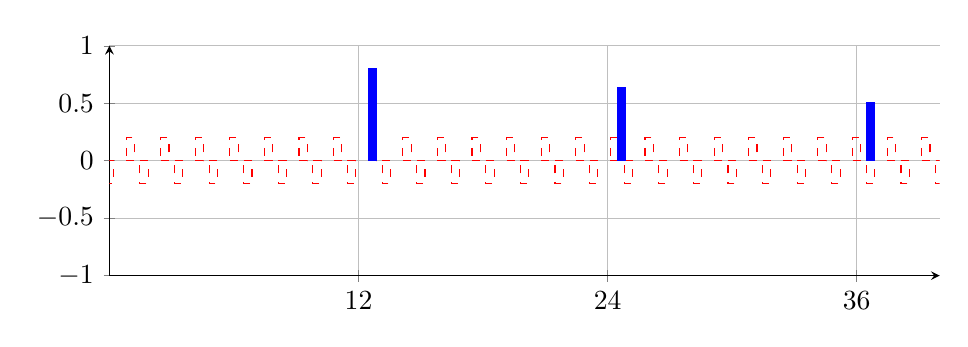
\begin{tikzpicture}
\begin{axis}[
    width=\textwidth, height=4.5cm,
    ymin=-1, ymax=1, xmin=0, xmax=40,
    ybar, bar width=3pt,
    xtick={12,24,36},
    grid=major,
    axis x line=bottom, axis y line=left
]
% Significance bands
\addplot[red, dashed, domain=0:40] {0.2};
\addplot[red, dashed, domain=0:40] {-0.2};
% Seasonal Lags (Exponential Decay)
\addplot[blue, fill=blue] coordinates {(12,0.8) (24,0.64) (36,0.51)};
\end{axis}
\end{tikzpicture}
\end{center}
\end{column}

\begin{column}{0.5\textwidth}
\begin{center}
\textbf{Theoretical PACF} \\
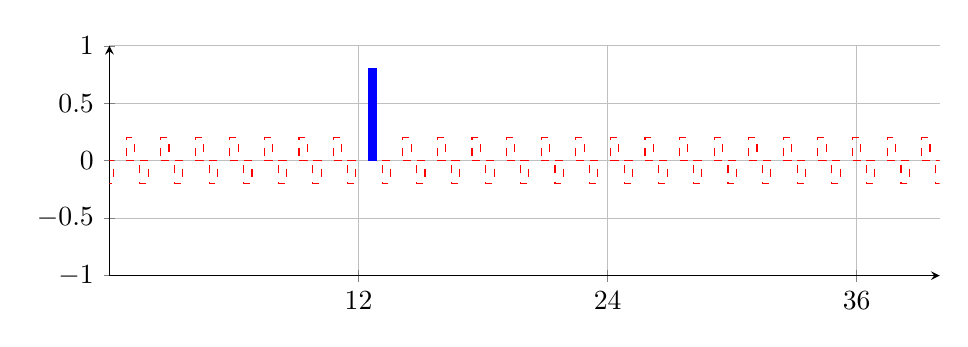
\begin{tikzpicture}
\begin{axis}[
    width=\textwidth, height=4.5cm,
    ymin=-1, ymax=1, xmin=0, xmax=40,
    ybar, bar width=3pt,
    xtick={12,24,36},
    grid=major,
    axis x line=bottom, axis y line=left
]
% Significance bands
\addplot[red, dashed, domain=0:40] {0.2};
\addplot[red, dashed, domain=0:40] {-0.2};
% Seasonal Lags (Sharp Cutoff)
\addplot[blue, fill=blue] coordinates {(12,0.8)};
\end{axis}
\end{tikzpicture}
\end{center}
\end{column}
\end{columns}

\vspace{0.2cm}
\begin{itemize}
    \item \textbf{Visual Rule:} PACF cuts off sharply after the first seasonal lag ($12$), while the ACF decays gradually across the seasonal multiples ($12, 24, 36$).
\end{itemize}
\end{frame}

\begin{frame}{Visualizing Seasonal Signatures: SMA(1) with $s=12$}
\textbf{Case 2: Pure Seasonal Moving Average Model ($Q=1$)}

\vspace{0.2cm}
\begin{columns}[T]
\begin{column}{0.5\textwidth}
\begin{center}
\textbf{Theoretical ACF} \\
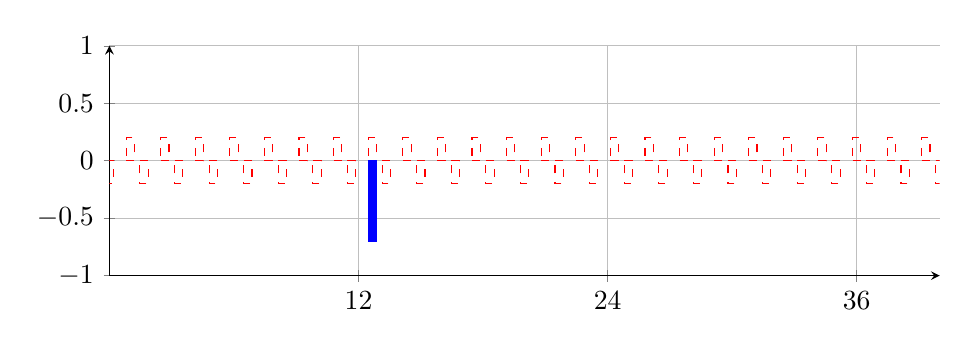
\begin{tikzpicture}
\begin{axis}[
    width=\textwidth, height=4.5cm,
    ymin=-1, ymax=1, xmin=0, xmax=40,
    ybar, bar width=3pt,
    xtick={12,24,36},
    grid=major,
    axis x line=bottom, axis y line=left
]
% Significance bands
\addplot[red, dashed, domain=0:40] {0.2};
\addplot[red, dashed, domain=0:40] {-0.2};
% Seasonal Lags (Sharp Cutoff)
\addplot[blue, fill=blue] coordinates {(12,-0.7)};
\end{axis}
\end{tikzpicture}
\end{center}
\end{column}

\begin{column}{0.5\textwidth}
\begin{center}
\textbf{Theoretical PACF} \\
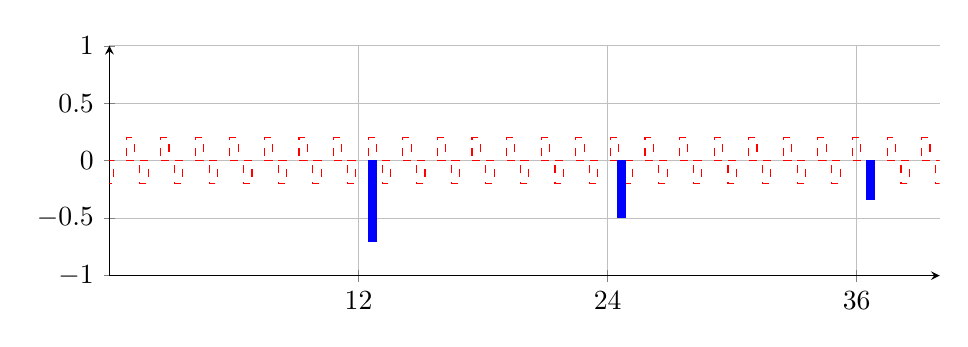
\begin{tikzpicture}
\begin{axis}[
    width=\textwidth, height=4.5cm,
    ymin=-1, ymax=1, xmin=0, xmax=40,
    ybar, bar width=3pt,
    xtick={12,24,36},
    grid=major,
    axis x line=bottom, axis y line=left
]
% Significance bands
\addplot[red, dashed, domain=0:40] {0.2};
\addplot[red, dashed, domain=0:40] {-0.2};
% Seasonal Lags (Decay)
\addplot[blue, fill=blue] coordinates {(12,-0.7) (24,-0.49) (36,-0.34)};
\end{axis}
\end{tikzpicture}
\end{center}
\end{column}
\end{columns}

\vspace{0.2cm}
\begin{itemize}
    \item \textbf{Visual Rule:} ACF cuts off sharply after the first seasonal lag ($12$), while the PACF decays gradually across the seasonal multiples.
\end{itemize}
\end{frame}

\begin{frame}{Visualizing Seasonal Signatures: SARMA(1,1) with $s=12$}
\textbf{Case 3: Mixed Seasonal Model ($P=1, Q=1$)}

\vspace{0.2cm}
\begin{columns}[T]
\begin{column}{0.5\textwidth}
\begin{center}
\textbf{Theoretical ACF} \\
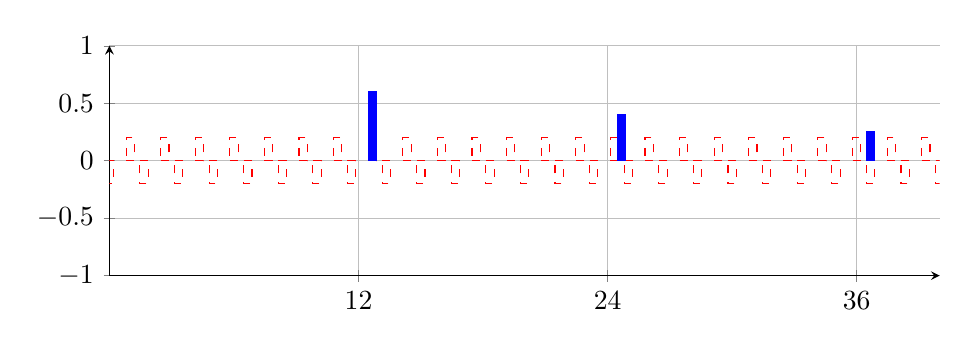
\begin{tikzpicture}
\begin{axis}[
    width=\textwidth, height=4.5cm,
    ymin=-1, ymax=1, xmin=0, xmax=40,
    ybar, bar width=3pt,
    xtick={12,24,36},
    grid=major,
    axis x line=bottom, axis y line=left
]
% Significance bands
\addplot[red, dashed, domain=0:40] {0.2};
\addplot[red, dashed, domain=0:40] {-0.2};
% Seasonal Lags (Decay)
\addplot[blue, fill=blue] coordinates {(12,0.6) (24,0.4) (36,0.25)};
\end{axis}
\end{tikzpicture}
\end{center}
\end{column}

\begin{column}{0.5\textwidth}
\begin{center}
\textbf{Theoretical PACF} \\
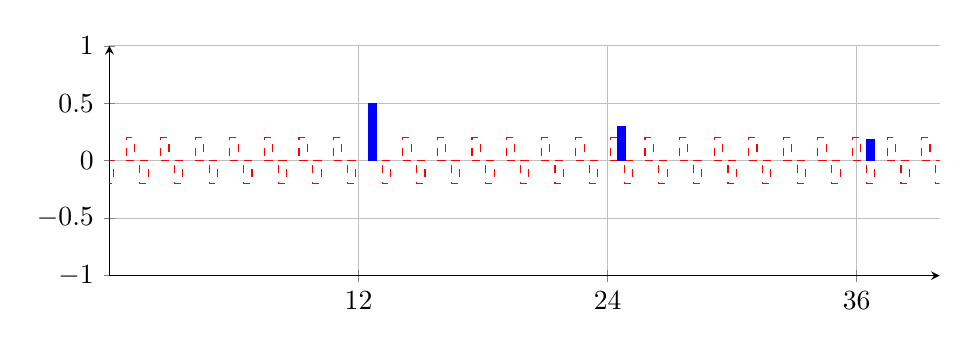
\begin{tikzpicture}
\begin{axis}[
    width=\textwidth, height=4.5cm,
    ymin=-1, ymax=1, xmin=0, xmax=40,
    ybar, bar width=3pt,
    xtick={12,24,36},
    grid=major,
    axis x line=bottom, axis y line=left
]
% Significance bands
\addplot[red, dashed, domain=0:40] {0.2};
\addplot[red, dashed, domain=0:40] {-0.2};
% Seasonal Lags (Decay)
\addplot[blue, fill=blue] coordinates {(12,0.5) (24,0.3) (36,0.18)};
\end{axis}
\end{tikzpicture}
\end{center}
\end{column}
\end{columns}

\vspace{0.2cm}
\begin{itemize}
    \item \textbf{Visual Rule:} Both ACF and PACF decay gradually across the seasonal multiples. No sharp cutoff at the seasonal lags.
\end{itemize}
\end{frame}

\begin{frame}{Testing for Seasonality: The Analytical Approach}
\textbf{Beyond Visual Inspection:}
\begin{itemize}
    \item While plotting the series and reading the ACF (looking for spikes at lags $s, 2s, 3s$) is the first step, we often need formal statistical proof that a seasonal pattern is significant and not just random noise.
    
    \vspace{0.3cm}
    
    \item \textbf{Three Main Approaches:}
    \begin{enumerate}
        \item \textbf{Regression-Based Tests:} Using seasonal dummy variables (ANOVA approach).
        \item \textbf{Non-Parametric Tests:} e.g., the Kruskal-Wallis test.
        \item \textbf{Seasonal Unit Root Tests:} e.g., the Canova-Hansen (CH) or OCSB tests (to determine if seasonal differencing $\Delta_s$ is strictly required).
    \end{enumerate}
\end{itemize}
\end{frame}

\begin{frame}{Statistical Proof: Seasonal Dummy Regression}
\textbf{The Intuition:} If seasonality exists, the mean of the series should vary significantly depending on the season (e.g., December average $\neq$ July average).

\vspace{0.2cm}

\textbf{1. The Model (Example for Monthly Data, $s=12$):}
\[
X_t = \alpha_0 + \gamma_1 D_{1,t} + \gamma_2 D_{2,t} + \dots + \gamma_{11} D_{11,t} + \varepsilon_t
\]
\begin{itemize}
    \item $D_{i,t}$ is a dummy variable that equals $1$ if time $t$ is in month $i$, and $0$ otherwise.
    \item We use $s-1$ dummies to avoid the \textit{dummy variable trap} (perfect collinearity).
\end{itemize}

\vspace{0.2cm}

\textbf{2. The Hypothesis Test (F-Test):}
\begin{itemize}
    \item \textbf{$H_0$:} $\gamma_1 = \gamma_2 = \dots = \gamma_{11} = 0$ (No deterministic seasonality).
    \item \textbf{$H_1$:} At least one $\gamma_i \neq 0$ (Seasonality is present).
    \item If the F-statistic is significant ($p$-value $< 0.05$), we reject $H_0$ and confirm the presence of a seasonal pattern.
\end{itemize}
\end{frame}

\begin{frame}{Formal Seasonal Unit Root Tests}
\textbf{Context:} Just as we use the ADF or KPSS tests to check for standard stationarity (and the need for $d$), we use specific tests to check for \textbf{seasonal stationarity} (and the need for $D$).

\vspace{0.3cm}

\begin{itemize}
    \item \textbf{The Canova-Hansen (CH) Test:}
    \begin{itemize}
        \item \textbf{Logic:} It is the seasonal equivalent of the KPSS test. 
        \item \textbf{$H_0$:} The seasonal pattern is stable and deterministic (No seasonal unit root $\implies$ Do NOT apply $\Delta_s$).
        \item \textbf{$H_1$:} The seasonal pattern is stochastic (Seasonal unit root exists $\implies$ Apply $\Delta_s$).
    \end{itemize}
    
    \vspace{0.3cm}
    
    \item \textbf{Practical Implementation in R/Python:}
    \begin{itemize}
        \item Algorithms like \texttt{auto.arima} or \texttt{pmdarima} run these tests under the hood automatically (e.g., using the CH or OCSB test) to decide whether $D$ should be $0$ or $1$ before searching for the $P$ and $Q$ parameters.
    \end{itemize}
\end{itemize}
\end{frame}

\begin{frame}[fragile]{Implementing Seasonal Dummy Regression}
\small
\textbf{Goal:} Test for deterministic seasonality using linear regression and an F-Test.

\vspace{0.2cm}

\begin{columns}[T]
\begin{column}{0.48\textwidth}
\begin{block}{R Implementation (\texttt{forecast})}
\begin{verbatim}
library(forecast)

# Assuming 'y' is a monthly ts object
# Generate s-1 seasonal dummies
dummies <- seasonaldummy(y)

# Fit the OLS model
fit <- lm(y ~ dummies)

# Check the F-statistic p-value
summary(fit) 
\end{verbatim}
\end{block}
\end{column}

\begin{column}{0.48\textwidth}
\begin{block}{Python Implementation (\texttt{statsmodels})}
\begin{verbatim}
import statsmodels.api as sm
import pandas as pd

# df has a monthly DatetimeIndex
# drop_first=True avoids dummy trap
dummies = pd.get_dummies(
    df.index.month, drop_first=True
).astype(int)

X = sm.add_constant(dummies)
fit = sm.OLS(df['value'], X).fit()

# Check the F-statistic p-value
print(fit.summary())
\end{verbatim}
\end{block}
\end{column}
\end{columns}
\end{frame}
\begin{frame}
\vspace{0.3cm}
\textbf{Interpretation:} If the overall F-statistic is significant ($p < 0.05$), we reject the null hypothesis and confirm the presence of a deterministic seasonal pattern.
\end{frame}

\begin{frame}[fragile]{Formal Seasonal Unit Root Tests ($D$)}
\small
\textbf{Goal:} Run formal tests (Canova-Hansen or OCSB) to mathematically determine if seasonal differencing ($D=1$) is required to achieve stationarity.

\vspace{0.2cm}

\begin{columns}[T]
\begin{column}{0.48\textwidth}
\begin{block}{R (\texttt{forecast} package)}
\begin{verbatim}
library(forecast)

# Assuming 'y' is a monthly ts object
# Run the Canova-Hansen Test
D_ch <- nsdiffs(y, test="ch")

# Run the OCSB Test
D_ocsb <- nsdiffs(y, test="ocsb")

print(D_ch)
# Output: 0 (No differencing needed) 
#         or 1 (Apply Delta_s)
\end{verbatim}
\end{block}
\end{column}

\begin{column}{0.48\textwidth}
\begin{block}{Python (\texttt{pmdarima} package)}
\begin{verbatim}
from pmdarima.arima.utils import nsdiffs

# data is a pandas Series
# m is the seasonal period (e.g., 12)

# Canova-Hansen Test
D_ch = nsdiffs(data, m=12, test='ch')

# OCSB Test
D_ocsb = nsdiffs(data, m=12, test='ocsb')

print(f"Seasonal differences: {D_ch}")
\end{verbatim}
\end{block}
\end{column}
\end{columns}
\end{frame}
\begin{frame}
\vspace{0.3cm}
\textbf{Note:} These functions directly return the recommended integer value for the seasonal difference parameter $D$ in your SARIMA$(p,d,q) \times (P,D,Q)_s$ model.
\end{frame}

\section{Volatility Models - Heteroscedasticity}

\begin{frame}{Limits of ARIMA Models}
\begin{itemize}
    \item \textbf{The Homoscedasticity Assumption:} Standard ARIMA models assume that the variance of the residuals (shocks) remains perfectly constant over time ($\text{Var}(\varepsilon_t) = \sigma^2$).
    
    \vspace{0.3cm}
    
    \item \textbf{The Reality of Financial Data:} In real-world financial series (e.g., stock returns, exchange rates), variance is rarely constant. The data frequently exhibits \textbf{Volatility Clustering}: periods of high turbulence are grouped together, followed by periods of relative calm.
    
    \vspace{0.3cm}
    
    \item \textbf{The ARIMA Blind Spot:} An ARIMA model is exceptionally good at forecasting the \textit{conditional mean} (the expected value), but it is completely blind to changes in the \textit{conditional variance} (the risk or uncertainty).
    
    \vspace{0.3cm}
    
    \item \textbf{The Solution:} To capture these dynamic shifts in risk, we must introduce a new family of non-linear models designed specifically for conditional heteroscedasticity: \textbf{ARCH} and \textbf{GARCH}.
\end{itemize}
\end{frame}

\begin{frame}{Stylized Facts of Financial Series}
\begin{itemize}
    \item \textbf{Volatility Clustering:} 
    \begin{itemize}
        \item As famously noted by Benoit Mandelbrot: \textit{"Large changes tend to be followed by large changes, of either sign, and small changes tend to be followed by small changes."}
        \item \textbf{Meaning:} Volatility comes in bursts. The variance of the series is autocorrelated; high turbulence today strongly predicts high turbulence tomorrow.
    \end{itemize}
    
    \vspace{0.4cm}
    
    \item \textbf{Conditional ($\sigma_t^2$) vs. Unconditional Variance ($\sigma^2$):} 
    \begin{itemize}
        \item \textbf{Unconditional Variance ($\sigma^2$):} The long-term, average variance over the entire dataset. For a stationary process, this remains constant.
        \item \textbf{Conditional Variance ($\sigma_t^2$):} The short-term, local variance at time $t$, given all available information up to time $t-1$. 
        \item \textbf{The Goal of ARCH/GARCH:} These models recognize that a series can be \textit{unconditionally homoscedastic} (stable long-term risk) but \textit{conditionally heteroscedastic} (dynamic short-term risk).
    \end{itemize}
\end{itemize}
\end{frame}

\section{The ARCH Model}

\begin{frame}{Intuition behind ARCH(q)}
\textbf{Conditional Variance Equation:}
\[
\sigma_t^2 = \alpha_0 + \sum_{i=1}^{q} \alpha_i \varepsilon_{t-i}^2
\]

\textbf{Modeling via Past Squared Errors:}
\begin{itemize}
    \item \textbf{Magnitude over Direction:} By squaring the past residuals ($\varepsilon_{t-i}^2$), the model reacts only to the \textit{size} of previous shocks, ignoring their sign. A massive market crash and a massive unexpected rally both lead to higher volatility tomorrow.
    
    \vspace{0.2cm}
    
    \item \textbf{Mathematical Volatility Clustering:} If recent periods experienced massive shocks ($\varepsilon_{t-1}^2$ is large), the weighted sum directly forces today's conditional variance ($\sigma_t^2$) to spike.
    
    \vspace{0.2cm}
    
    \item \textbf{The Baseline Risk:} $\alpha_0$ represents the baseline, minimum level of volatility that exists in the market even when all recent shocks are zero.
\end{itemize}
\end{frame}

\begin{frame}{Conditions for Validity in ARCH(q)}
\textbf{To ensure the model is mathematically valid and financially realistic:}

\vspace{0.2cm}
\begin{itemize}
    \item \textbf{Positivity Constraints:} 
    \begin{itemize}
        \item By definition, a variance ($\sigma_t^2$) can never be negative.
        \item To guarantee this under any realization of past shocks, the parameters must be strictly positive: $\alpha_0 > 0$ and $\alpha_i \ge 0$ for all $i$.
    \end{itemize}
    
    \vspace{0.4cm}
    
    \item \textbf{Condition for Finite Unconditional Variance (Stationarity):}
    \begin{itemize}
        \item While the \textit{conditional} variance fluctuates daily, the overall process must still have a stable, long-term \textit{unconditional} variance ($\sigma^2 = \frac{\alpha_0}{1 - \sum \alpha_i}$).
        \item \textbf{Mathematical Requirement:} 
        \[ \sum_{i=1}^{q} \alpha_i < 1 \]
        \item \textbf{Consequence of violation:} If $\sum \alpha_i \ge 1$, a single shock would cause the variance to cascade and grow infinitely over time, which is financially impossible.
    \end{itemize}
\end{itemize}
\end{frame}
\section{The GARCH Model}

\begin{frame}{Why Generalize ARCH?}
\begin{itemize}
    \item % To be completed: Parsimony problem (too many parameters in ARCH)
    \item % To be completed: Introducing volatility memory
\end{itemize}
\end{frame}

\begin{frame}{Focus on GARCH(1,1)}
\textbf{Equation:}
\[
\sigma_t^2 = \alpha_0 + \alpha_1 \varepsilon_{t-1}^2 + \beta_1 \sigma_{t-1}^2
\]

\begin{itemize}
    \item % To be completed: Interpretation of ARCH and GARCH terms
\end{itemize}
\end{frame}

\begin{frame}{Stationarity Condition for GARCH(1,1)}
\textbf{Condition:}
\[
\alpha_1 + \beta_1 < 1
\]

\begin{itemize}
    \item % To be completed: What happens if the sum approaches 1 (persistence)?
\end{itemize}
\end{frame}

\begin{frame}{Practical Diagnostics}
\begin{itemize}
    \item % To be completed: Engle's LM Test on squared residuals
    \item % To be completed: Practical implementation
\end{itemize}
\end{frame}

\end{document}